\chapter{Tokenizer properties affect the performance of language models}
\label{chap:experiment_1_validity}

% \textbf{Q1:} How do subword tokenizers differ in overlap and allocation of learned vocabularies?
% \textbf{Q2:} Which properties of multilingual tokenizers affect the language model representation quality?

% motivation
In this chapter, we propose and conduct an experiment to answer (\textbf{Q1}) how subword tokenizers differ in overlap and allocation of learned vocabularies. Moreover, we explore (\textbf{Q2}) which properties affect the language model representation quality. Our goal is to establish that the metrics we propose are useful for assessing the differences between tokenizers and that they are useful for comparing whether a given tokenizer is better than another.

% overview
To answer these questions, we train three tokenizers and assess how they differ in the metrics we propose. We then look at how are these differences manifested when we use these tokenizers to train otherwise identical multilingual models. We then assess whether the proposed metrics are good predictors of the model's performance.

The results presented in this section are selected from our paper \citet{limisiewicz_tokenization_2023}. We refer the reader to the paper for more in-detail analysis and additional experiments. Here we present experiments that are most relevant to the thesis goal.

% method
\section{Analysis of Tokenizer Properties}

We train three distinct tokenizers --- Huggingface Unigram, Huggingface BPE and TokMix tokenizer \cite{limisiewicz_tokenization_2023} described in the following subsection. We use the Huggingface implementation\footnote{\href{https://github.com/huggingface/tokenizers}{https://github.com/huggingface/tokenizers}} of the training algorithms for the Unigram and BPE tokenizers. The training data for all tokenizers is the CC100 corpus sampled with the exponential smoothing factor $\alpha=0.25$.
% which corresponds to the XLM-R tokenizer (there $\alpha=0.3$). 
After tokenizer training, we perform an intrinsic evaluation of the tokenizers on each language separately and report the macro average of the metrics (For details see \autoref{sec:intrinsic_evaluation}).

After tokenizer evaluation, we use the tokenizers to train three masked language models. We use the same training data and the same model architecture for all models defined in \autoref{sec:model_pretraining}. The only difference is the tokenizer used to preprocess the data. We then evaluate the models using probing on three multilingual word-level tasks (part of speech tagging, dependency labeling and named entity recognition) and one sentence-level task (cross-lingual natural language inference).
We evaluate the overall in-language performance and compare it to the tokenizer metrics. We then do a more fine-grained comparison by evaluating the model on each language separately and comparing the results to the tokenizer metrics also measured on each language separately. (For details see \autoref{sec:extrinsic_evaluation}) 



% and then we assess 

% which we explain in 

\subsection{TokMix tokenizer}

To create our TokMix tokenizer, we run the Huggingface Unigram tokenizer training on each language corpus $C_l, l \in L$ separately. After this, we end up with 20 separate tokenizers with equal vocabulary sizes. We merge the vocabularies of all tokenizers into one large vocabulary $V = \bigcup_{l \in L} V_l$, average the token probabilities and trim the vocabulary to the desired size $|V| = 120\,000$. 

\section{Results}
\subsection{Intrinsic evaluation}

\begin{table}
\caption{In the first batch of experiments, we compare the Huggingface Unigram, Huggingface BPE, and our TokMix method based on merging Huggingface Unigram tokenizers. Huggingface Unigram has significantly lower vocabulary allocation scores ($-0.4$ CPT and $-153$ AR) than BPE and TokMix. This means that Unigram uses shorter tokens and the capacity of the vocabulary is used less uniformly. Moreover, the vocabulary has more overlap (JSD decrease by $-0.03$) between the languages for Unigram.  The scores are macro averages over all languages, computed over a holdout portion of the CC100 corpus. We sample 10k lines from each language which we have empirically found to be enough to get representative results.}
\label{tab:20l_metrics}
\begin{tabular}{lrrrrr}
\toprule
Tokenizer & Alphabet & \# UNKs & CPT & AR & JSD \\
\midrule
huggingface\_bpe\_alpha0.25 & 1000 & 14040.1 & 3.713 & 1253.7 & 0.783 \\
TokMix\_alpha0.25 & 2497 & 1203.2 & 3.691 & 1163.4 & 0.773 \\
huggingface\_unigram\_alpha0.25 & 12616 & 4.5 & 3.204 & 1010.5 & 0.745 \\
\bottomrule
\end{tabular}
\end{table}


In the \autoref{tab:20l_metrics} we see that the choice of the tokenization method largely influences the vocabulary allocation and overlap metrics. The Huggingface BPE tokenizer produces on average the longest tokens (high CPT), the most uniform allocation of tokens (high AR), and the least overlap between languages (high JSD). On the other hand, the Huggingface Unigram segments the text into shorter tokens and the average vocabulary overlap between all languages is much higher. The high overlap might be related to the low allocation as it is more likely that shorter tokens are shared between languages. 

Interestingly, the TokMix tokenizer has a similar \textit{vocabulary allocation} (CPT, AR) as the Huggingface BPE tokenizer. This is surprising as the TokMix tokenizer is based on the Huggingface Unigram tokenizer, which shows significantly lower scores.

\subsection{Extrinsic evaluation}

% Next, we use the tokenizers from \autoref{tab:20l_metrics} and pretrain three masked language models with otherwise identical configuration and training data.
% We then evaluate the quality of the output representations of these models by probing the contextualized vectors against several tasks (XNLI, UD, POS, NER). We test the in-language and cross-lingual settings. The in-language setting are shown in \autoref{fig:pair_analysis_20L}. We show the relationship between our metrics and the downstream tasks.
Next, we use the tokenizers from \autoref{tab:20l_metrics} and pretrain three masked language models. We find that the choice of the tokenizer has a large impact on the model's in-language performance. The \autoref{tab:in_lang_avg_20l} shows that the Huggingface Unigram has a significantly lower performance than the other two tokenizers on the word-level tasks (NER, POS, UD). The overall performance on sentence-level NLI is similar across tokenizers. % We see a similar trend for the cross-lingual setting

We validate this observation by looking at the interaction between the tokenizer metrics and model performance on the level of individual evaluation languages \autoref{fig:pair_analysis_20L}. In each scatterplot, each point represents a pair $(\tau, l)$ of a tokenizer $\tau$ from our three tested tokenizers and a language $l$ from the set of languages available for the given task. The position of the point corresponds to the observed tokenizer metrics and task performance \footnote{As explained in \autoref{sec:correlation_intrinsic_extrinsic}, we center the tokenizer metrics and downstream task results by subtracting the mean for each language to account for the differences between languages we cannot control for. This way we see only the improvements and deteriorations of the tokenizers and models compared to the mean value for the given language.}.
% %  \xxx{ohh, maybe better would be not to plot the whole scattermatrix but only 2x3 table with AR,CPT vs NER,POS,NLI} 
%  \tomasz{I agree, but change it only if you have enough time!}
  We see that the Huggingface Unigram tokenizer exhibits lower performance on the word-level tasks (NER, POS, UD) which corresponds to the lower vocabulary allocation metrics. We the most clear relationship between NER and CPT, UD and CPT, and POS and CPT. We quantify this relationship by computing Spearman's correlation coefficient between the tokenizer metrics and the model performance. The results are shown in \autoref{tab:corr_in_lang_20l}. We see that the vocabulary allocation metrics are positively correlated with the model performance on the word-level tasks. The length of the tokens has a strong positive influence on POS, dependency labeling, and NER results ($r > 0.65$), while it does not significantly affect NLI results. The correlation between the average rank and NER scores is weaker but still significant. Moreover, it is significantly correlated with XNLI accuracy with a medium coefficient $r = 0.56$. Our findings suggest that longer tokens and more tokens allocated for a given language in the vocabulary improve the in-language model performance on our tested tasks. 

We conduct a similar analysis for the cross-lingual setting. We evaluate the probes on all languages except the one on which the probe was trained on. The results are shown in \autoref{fig:X_pair_analysis_20L} and a summary of the correlations in \autoref{tab:corr_x_lang_20l}. Each point corresponds to a triplet $(\tau, l_\mathrm{src}, l_\mathrm{tgt})$ of a tokenizer $\tau$, a language $l_\mathrm{src}$ the probe was trained on, and a language $l_\mathrm{tgt} \neq l_\mathrm{src}$ the probe was evaluated on. We see that the cross-lingual performance is positively correlated with the vocabulary overlap metric JSD in the case of the word-level tasks. This suggests that smaller vocabulary overlap between the languages improves the cross-lingual performance on the word-level tasks. On the other hand, we see that the correlation between the combined CPT metric and the cross-lingual performance is similarly strong and that there is also a strong correlation between JSD and combined CPT. In this case, the correlation between JSD and downstream performance could be caused by a confounding factor of better vocabulary allocation as measured by CPT.

Overall, we see that the differences between tokenizers are reflected in the representation quality. High CPT and AR metrics are correlated with better probe performance, especially on word-level tasks such as part of speech tagging, named entity recognition, and dependency labeling. Moreover, the cross-lingual performance is also correlated with the vocabulary allocation and overlap metrics. 

Therefore, we see that our metrics are useful for assessing the differences between tokenizers. Moreover, the differences in tokenizers are reflected in the learned representations of the models, especially on word-level tasks.

~

Note that in this section we have included only a part of the experiments from our paper \citet{limisiewicz_tokenization_2023} published in ACL Findings 2023. Namely, we focus only on the experiments that are based on the same 20 languages as the rest of the thesis. For our purposes, we focus only on the more general conclusions. We refer the reader to the original paper for the full set of experiments, where we additionally discuss in more detail which tasks are more affected by which properties of the tokenizers.



% The probe performance is largely dependent on the tested language, to assess only the differences yielded by the use of different tokenizers, \tomaszrep{we center the per-language results on the mean across the three models}{we center results, i.e. substract mean across the tree models from per language results}.
%  This way we see only the improvements and deteriorations of the models compared to the mean performance. The metrics are centered in the same way. 


% \xxx{maybe I can actually get rid of the scatterplots and just show the correlation tables from the paper. The problem is the mixing of 6 langs and 20 langs which I do not explain here.} \tomasz{can we just keep 20 languages results?}

% All correlations are summarized in \autoref{tab:corr_in_lang_20l} and \autoref{fig:corr_x_lang_20l}. The length of the tokens has a strong positive influence on POS, dependency labeling, and NER results ($r > 0.65$), while it does not significantly affect NLI results. The correlation between the average rank and NER scores is weaker but still significant. Moreover, it is significantly correlated with XNLI accuracy with a medium coefficient $r = 0.56$. 

% Overall, we see that our metrics are useful for assessing the differences between tokenizers. Moreover, the differences in tokenizers are reflected in the learned representations of the models, especially on word-level tasks.

% \xxx{what to do with JSD, in paper we present the 6 lang experiments. Here I wanted to keep things simple and focus on the 20 lang experiments. But it seems that for 20 langs the influence of JSD is actually positive for NER and there is $\approx 0$ influence on XNLI. }\tomasz{I think lack of correlation is caused by not trying NoOverlap method for 20 languages. Consider skipping this finding.}

% Firstly, we see that the default settings of the Huggingface tokenizers produce very different alphabet sizes and in turn affect the UNK rate. As we will see later, this does not affect the metrics significantly.

\begin{table}
\centering
\caption{Results of extrinsic evaluation for the Huggingface tokenizers. We observe significant changes for different tokenization methods. We report the F1 score for NER, POS and UD. XNLI is reported as accuracy. The scores are macro averages over all languages.}
\label{tab:in_lang_avg_20l}
    \small
    \begin{tabular}{llllllll}
    \toprule
    Tokenizer    &               NER &               POS &                UD &              XNLI \\
    \midrule
    Huggingface BPE       &  66.3 $_{\pm0.2}$ &  67.3 $_{\pm0.4}$ &  54.5 $_{\pm0.5}$ &  53.5 $_{\pm0.3}$ \\
    TokMix    &  65.4 $_{\pm0.3}$ &  66.5 $_{\pm0.4}$ &  53.9 $_{\pm0.5}$ &  52.3 $_{\pm0.3}$ \\
    Huggingface Unigram   &  58.9 $_{\pm0.2}$ &  54.0 $_{\pm0.4}$ &  43.7 $_{\pm0.4}$ &  53.2 $_{\pm0.3}$ \\
    \bottomrule
    \end{tabular}
\end{table}

\begin{figure}
    \centering
    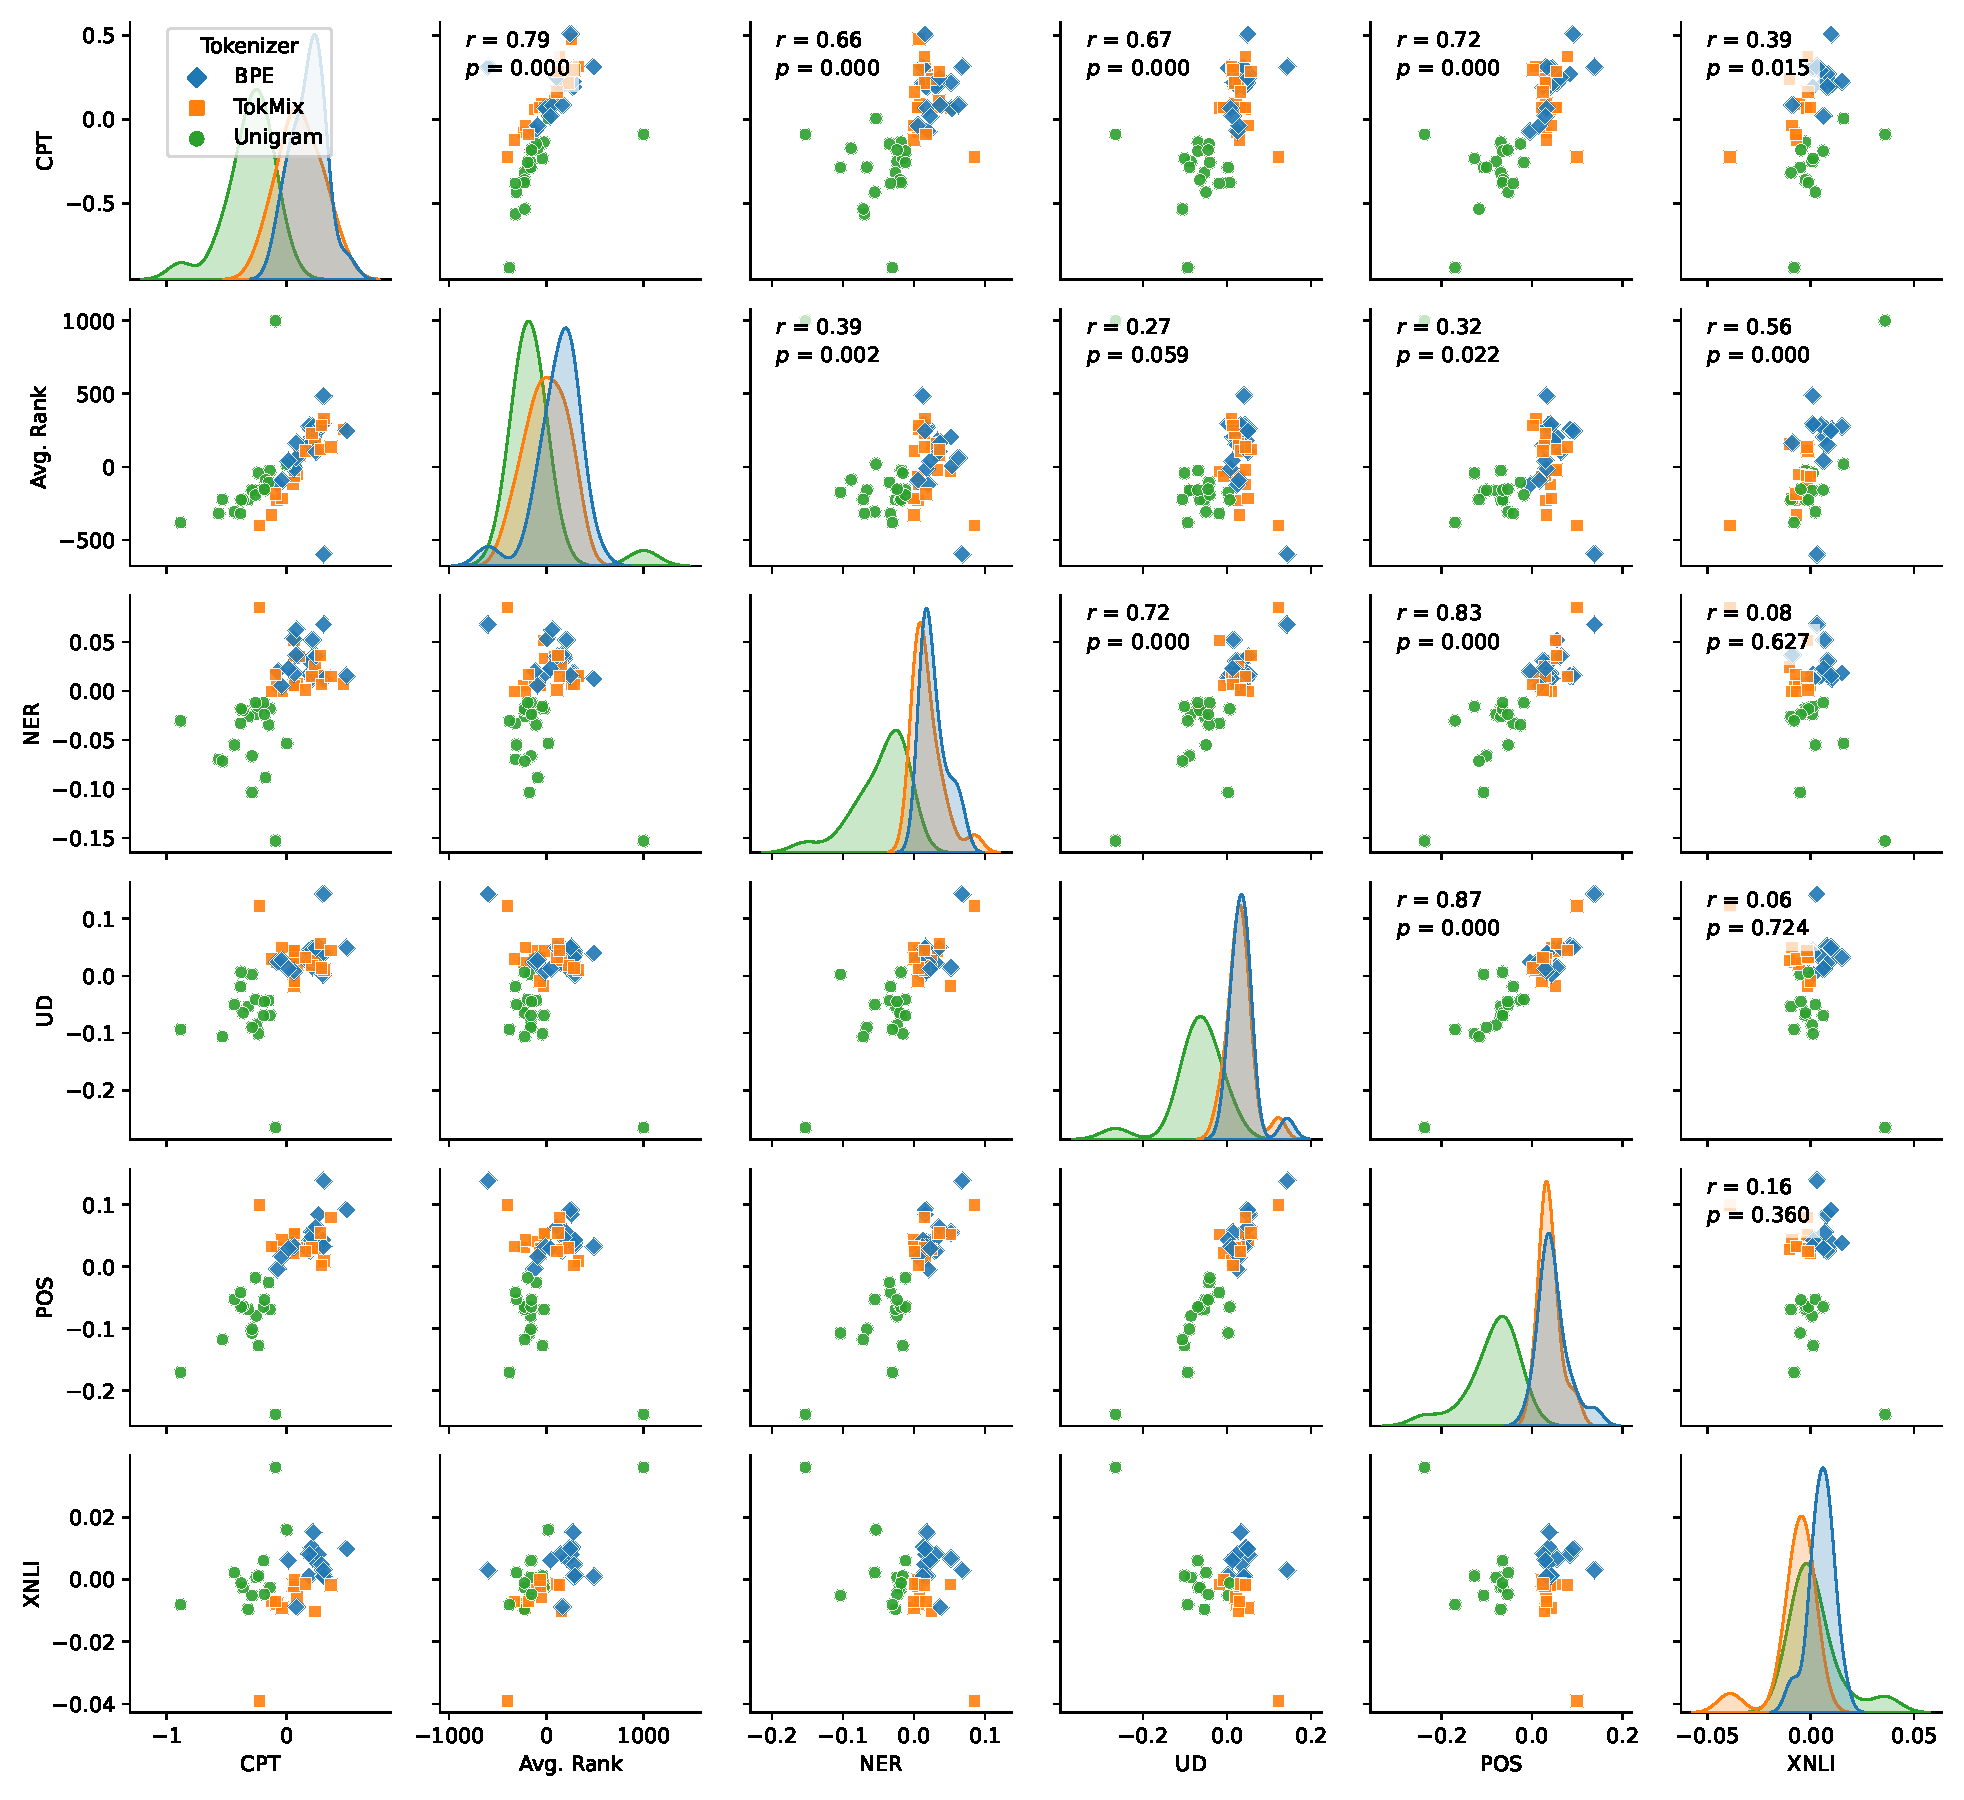
\includegraphics[width=\textwidth]{figures/pair_analysis_20L.pdf}
    \caption{We compare the tokenizer metrics against the contextualized representation quality. For each tokenizer, we pretrain a masked language model, freeze it, and train a linear probe for each task and each of the available languages. We observe a high Spearman correlation between CPT and the word-level tasks (NER, POS, UD) and a high correlation between AR and the sentence-level task XNLI. This suggests that our vocabulary allocation metrics are good indicators of the tokenizer's quality and higher vocabulary allocation leads to better downstream performance. Each data point corresponds to an average result over three seeds of probe training and evaluating one of the languages. The results for each language are centered around the mean to account for the differences between languages as explained in \autoref{sec:correlation_intrinsic_extrinsic}. The colors of points are assigned for specific tokenizers.}
    \label{fig:pair_analysis_20L}
\end{figure}

\begin{figure}
    \centering
    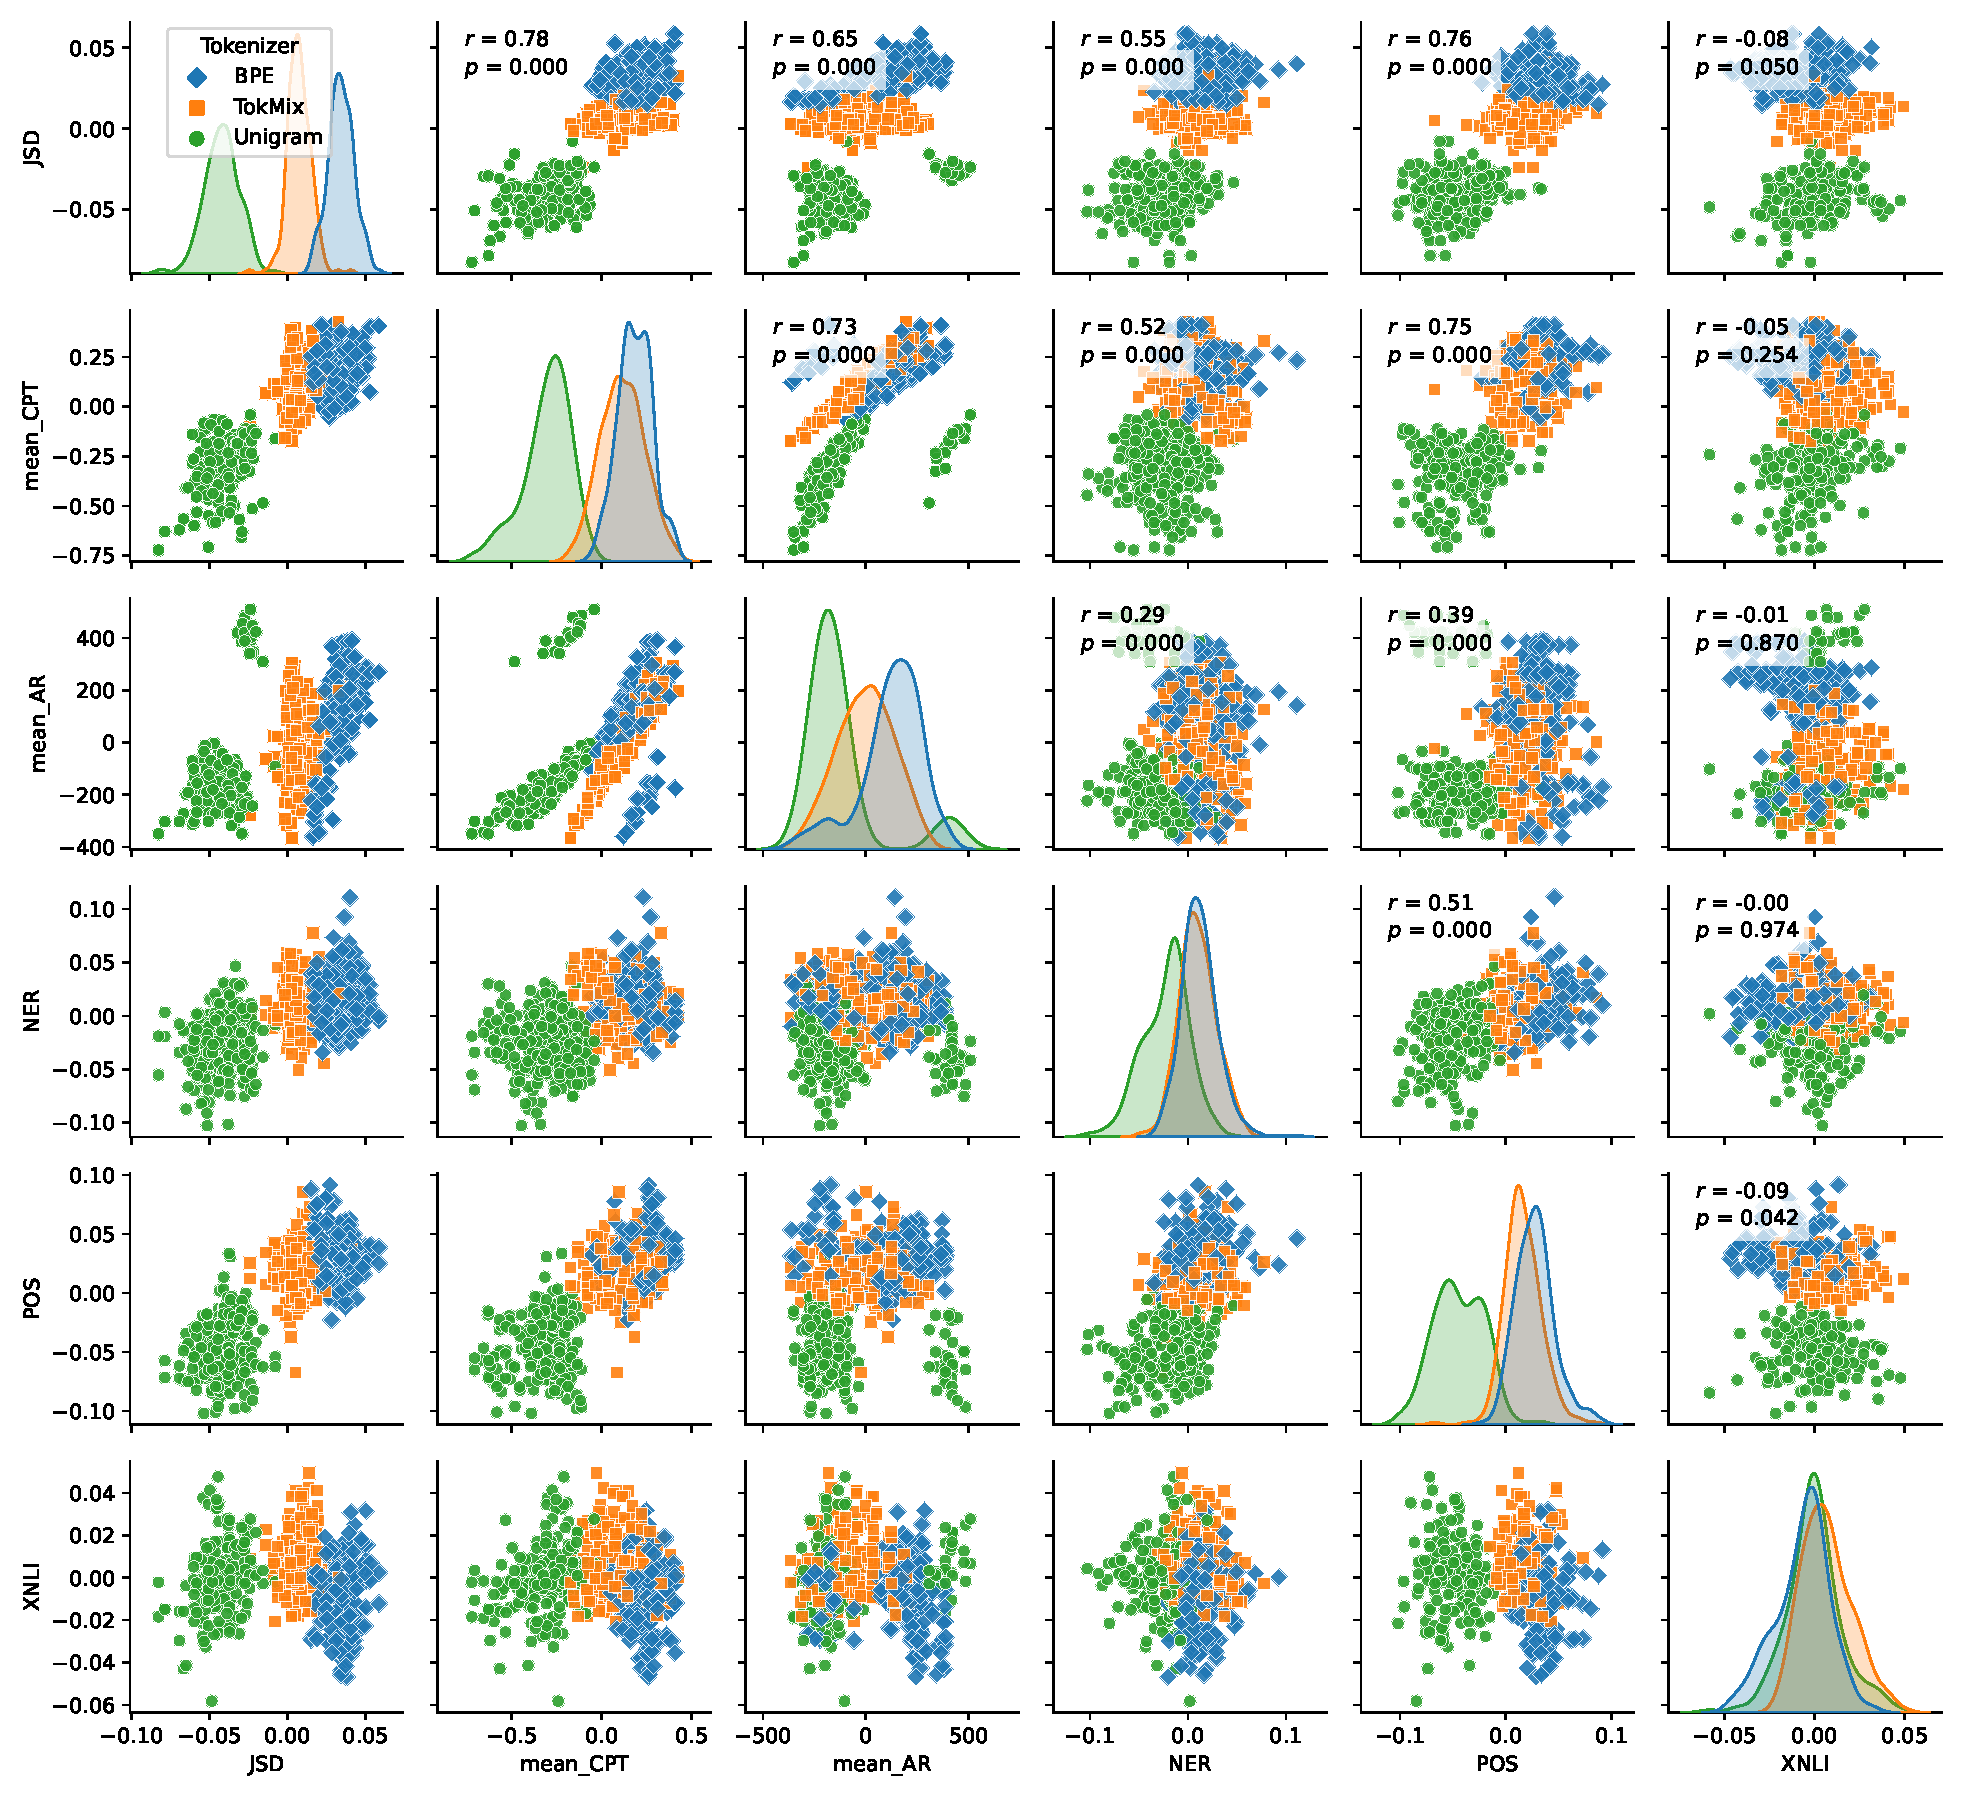
\includegraphics[width=\textwidth]{figures/X_pair_analysis_20L.pdf}
    \caption{We compare the tokenizer metrics against the cross-lingual performance of the models. For each tokenizer, we pretrain a masked language model, freeze it, and train a linear probe on each of the available languages. Then we evaluate the models on all languages the probe has \textbf{not} been trained on, assessing the cross-lingual properties of the model. Here we observe a high correlation between JSD and the word-level tasks, especially the POS and UD. This suggests that less overlap (higher divergence) between the vocabularies of the languages leads to better cross-lingual performance for word-level tasks.} 
    \label{fig:X_pair_analysis_20L}
\end{figure}

\begin{table}
\centering

\begin{tabular}{lcc}
\toprule
 & \multicolumn{2}{c}{\bf{V. Allocation}} \\
 & (AR) &  (CPT) \\
\midrule
CPT    &    \bf{0.790} &     - \\
NER    &   \bf{0.394} &   \bf{0.657}  \\
POS    &     0.320 &   \bf{0.724} \\
Dep l. &     0.266 &   \bf{0.675} \\
NLI   &    \bf{0.56} &    0.388 \\ 
\bottomrule
\end{tabular}
\caption{Spearman correlations between centered in-language task results and tokenizer measures. Statistically significant correlations ($p<0.01$) are bolded.}
\label{tab:corr_in_lang_20l}
\end{table}
\begin{table*}
\centering
\begin{tabular}{lcccccc}
\toprule
 & \bf{V. Overlap} & \multicolumn{2}{c}{\bf{V. Allocation SRC}}  & \multicolumn{2}{c}{\bf{V. Allocation TGT}} \\ 
 & (JSD) &  (AR)  &  (CPT) & (AR) & (CPT) \\ \midrule
% NER     &  \bf{-0.153} &        0.061 &  \bf{0.174} &   \bf{0.180} &   \bf{0.250} \\
% POS     &   \bf{0.164} &       \bf{0.187} &  \bf{0.366} &       \bf{0.238} &  \bf{0.379} \\
% Dep l.     &   \bf{0.095} &      \bf{ 0.095} &  \bf{0.216} &       \bf{0.134} &  \bf{0.232} \\
% NLI    &  \bf{-0.234} &         -0.060 &   -0.025 &       -0.079 &   -0.071 \\
% Retrieval &  \bf{-0.157} &         0.041 &    0.023 &         0.031 &     0.020 \\
NER     &  \bf{0.553} &       \bf{0.172} &  \bf{0.412} &      \bf{0.409} &  \bf{0.568} \\
POS     &  \bf{0.759} &       \bf{0.383} &   \bf{0.69} &       \bf{0.436} &  \bf{0.714} \\
Dep l.     &  \bf{0.596} &       \bf{0.314} &  \bf{0.587} &       \bf{0.351} &  \bf{0.605} \\
NLI    &  -0.078 &        -0.039 &   -0.006 &       -0.083 &  -0.082 \\
Retrieval &  \bf{0.156} &       \bf{0.214} &  \bf{0.139} &       \bf{0.214} &  \bf{0.144} \\
\bottomrule
\end{tabular}
\caption{Spearman correlations between cross-lingual transfer results and tokenization measures. vocabulary overlap~is measured by JSD, we also measure the correlation with vocabulary allocation s of source and target language of the transfer directions. Statistically significant correlations ($p<0.01$) are bolded. Computed for 20 languages.}
\label{tab:corr_x_lang_20l}
\end{table*}


% \tomasz{I suggest a short section Conclusion/Findings recapitulating the main observations in contex of the research questions.}

\section{Findings}

% \textbf{Q1:} How do subword tokenizers differ in overlap and allocation of learned vocabularies?
% \textbf{Q2:} Which properties of multilingual tokenizers affect the language model representation quality?

We find that the choice of the tokenization method largely influences the vocabulary allocation and overlap metrics (\textbf{Q1}). We see that Huggingface BPE better allocates the vocabulary overall and has a lower overlap between languages. On the other hand, the Huggingface Unigram tokenizer segments the text into shorter tokens and the average vocabulary overlap between all languages is much higher.

We find that the differences between tokenizers are reflected in the representation quality (\textbf{Q2}). High vocabulary allocation metrics are correlated with better probe performance, especially on the word-level tasks. Moreover, the cross-lingual performance is correlated with higher vocabulary allocation and lower overlap.

Our findings validate our proposed metrics as they are useful predictors of the model's performance.